\section{Common Notation Mistakes}
\label{sec:common-manuscript-mistakes}
Notation follows a strict set of rules and conventions, however there are a \emph{lot} of them and as such it's perfectly natural that children struggle to remember them all, resulting in mistakes.

In order to focus the scope of this dissertation, I needed to establish exactly which mistakes were most likely to occur. In order to understand what these might be, I referred to two main sources.

The first is Music Theory in Practice, \parencite{taylor2008music}  This book, written specifically to assist those teaching music theory, has some good examples of mistakes a student should avoid.

The second is consultation with professional musicians and teachers. This is covered further in \cref{sec:teacher-data-gathering}.

\subsection{Gathering Professional Feedback}
\label{sec:teacher-data-gathering}

In order to build an application which can help to compensate for the absence of a tutor, we need to ensure that it can spot as many of the same mistakes as a tutor would.

The most logical way to establish precisely what these mistakes might be is to ask the tutors. When I did this, several of them found it difficult to express the mistakes they had seen children make without a piece of music in front of them.

I therefore devised the following method for gathering data to form a `mistake database'.

\begin{enumerate}
  \item Build the input section of the application such that a student can `free-draw' on a blank music staff.
  \item Set the student challenges and ask them to have a go at as many as they can
  \item Print out the attempts (labelled) and get a music tutor to mark them freehand
  \item Collate and summarise the feedback
\end{enumerate}

To save time (and paper) the marking was done 3-UP on a portrait sheet of A4, an example of one of the tutor feedback sheets can be seen in \cref{fig:teacher-sheet}. It should be noted that in some of the feedback tutors refer to errors differently, for example by using `the stem is on the wrong side' to mean that either a note stem is up when it should be down or that it's on the right when it should be on the left. Below are annotated examples of the mistakes \noteED needs to be able to identify.

\begin{figure}[H]
  \centering
  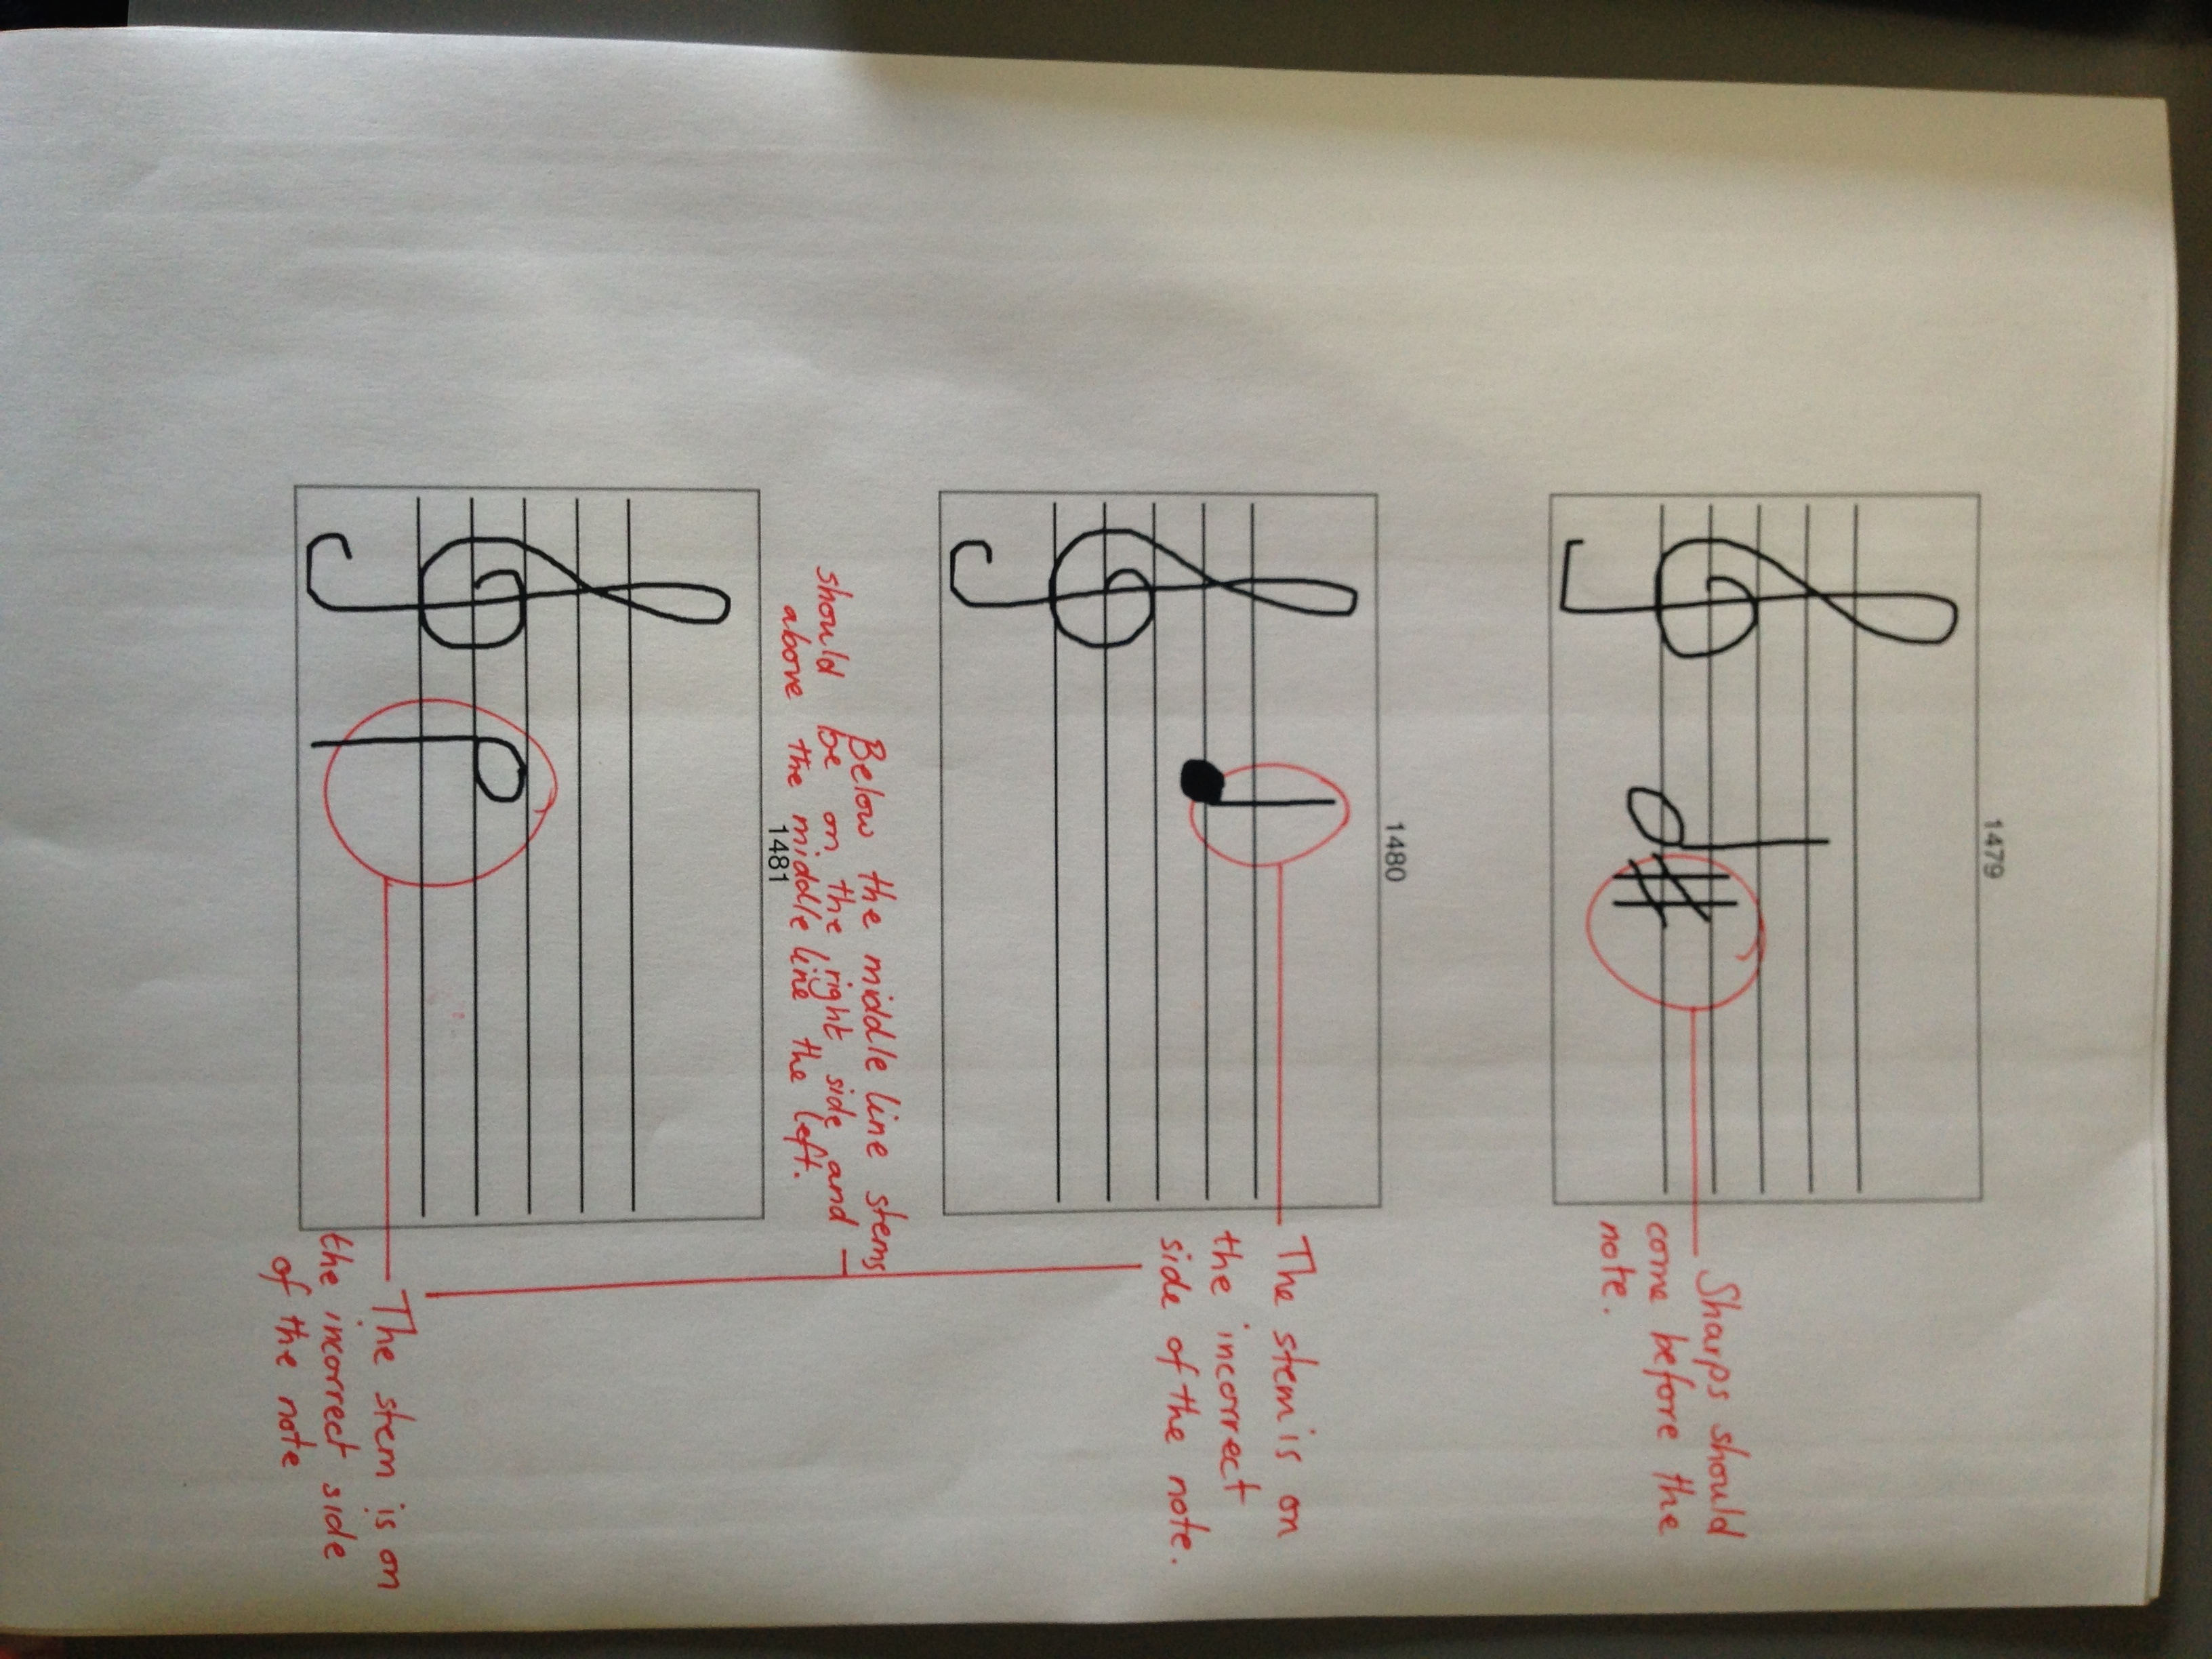
\includegraphics[width=\linewidth]{gfx/photos/teacher-sheet-1.jpg}
  \caption{Example of tutor-annotated manuscript}
  \label{fig:teacher-sheet}
\end{figure}

Once this data was collected I had a sample of 83 attempts at various notation challenges, of which a number were annotated. I was then able to extract some of the recurring issues which \noteED should aim to recognise which I've summarised in \cref{table:teacher-feedback-summary}. I present what is by no means an exhaustive list below and later on in \cref{sec:scoring} I go over how I actually identify, score and provide feedback to the student for these mistakes.

\begin{table}[H]
    \centering
    \begin{tabularx}{\textwidth}{ llll }
        \toprule

        Element & Issue & Description & Analysis \\
        \midrule
        Note Head       & Ambiguous Position     & \cref{sec:tf-note-head-ambiguous}              & \cref{sec:scoring-position} \\
        Note Head       & Broken Lines           & \cref{sec:tf-note-head-broken}            & \cref{sec:scoring-note-head-broken} \\
        Note Head       & Angled                 & \cref{sec:tf-semibreve-angled}            & \cref{sec:scoring-semibreve-angled} \\
        Note Head       & Messy                  & \cref{sec:tf-note-head-messy}             & \cref{sec:scoring-note-head-messy} \\
        Stem            & Length                 & \cref{sec:tf-stem-length}                 & \cref{sec:scoring-stem-length} \\
        Stem            & Straightness           & \cref{sec:tf-stem-straightness}           & \cref{sec:scoring-stem-straightness} \\
        Stem            & Direction              & \cref{sec:tf-stem-direction}              & \cref{sec:scoring-stem-direction} \\
        Stem            & Side                   & \cref{sec:tf-stem-side}                   & \cref{sec:scoring-stem-side} \\
        Stem            & Angle                  & \cref{sec:tf-stem-angle}                  & \cref{sec:scoring-stem-angle} \\
        Quaver Tail     & Side                   & \cref{sec:tf-quaver-tail-side}            & \cref{sec:scoring-quaver-tail-side} \\
        Rest            & Position               & \cref{sec:tf-rest-position}               & \cref{sec:scoring-position} \\
        Accidental      & Ambiguous Position     & \cref{sec:tf-accidental-ambiguous}        & \cref{sec:scoring-position} \\
        Key Signature   & Incorrect Octave       & \cref{sec:tf-keysig-octave}               & \cref{sec:scoring-keysig-octave} \\
        Key Signature   & Incorrect Ordering     & \cref{sec:tf-keysig-order}                & \cref{sec:scoring-keysig-order} \\
        Key Signature   & Incorrect Accidentals  & \cref{sec:tf-keysig-incorrect}            & \cref{sec:scoring-keysig-incorrect} \\
        Beats \& Timing & Too Many Beats         & \cref{sec:tf-beats-too-many}              & \cref{sec:scoring-beats}\\
        Beats \& Timing & Too Few Beats          & \cref{sec:tf-beats-too-few}               & \cref{sec:scoring-beats}\\
        \bottomrule
    \end{tabularx}
    \caption{A brief summary of some mistakes which emerged from the preliminary data gathering. `FUTURE' indicates that analysis for the mistake hasn't yet been incorporated into the application}
    \label{table:teacher-feedback-summary}
\end{table}

\subsection{Note Heads}
\subsubsection{Ambiguous Position}\label{sec:tf-note-head-ambiguous}

The semibreve is the easiest note to draw and is simply an oval outline, however, the rules which govern it's placement are quite specific as outlined in Figures \cref{fig:semibreve-on-line} \& \cref{fig:semibreve-on-space}

\begin{figure}[width=.8\textwidth][h!]
  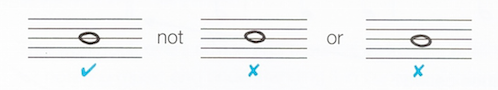
\includegraphics[width=\linewidth]{gfx/basic/semibreve-on-line.png}
  \centering
  \caption{If it is drawn on the line, the line must go exactly through the middle of the semibreve}
  \label{fig:semibreve-on-line}
\end{figure}


\subsubsection{Too Big/Small}\label{sec:tf-note-head-scale}

\begin{figure}[H]
  \centering
  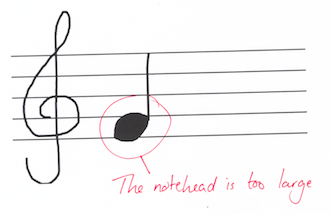
\includegraphics[width=.4\linewidth]{gfx/teacher-notes/mistake-notehead-too-big.png}
  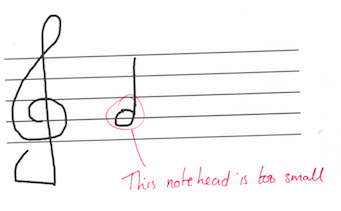
\includegraphics[width=.4\linewidth]{gfx/teacher-notes/mistake-notehead-too-small.png}
  \caption{Note heads should be one staff space in size and not extend beyond a pair of staff lines}
  \label{fig:mistake-note-ambig}
\end{figure}

\begin{figure}[h!]
  \centering
  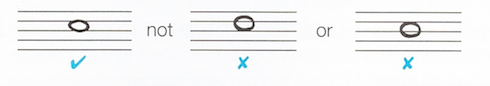
\includegraphics[width=\linewidth]{gfx/basic/semibreve-on-space.png}
  \caption{If it is drawn in the space, it should only cover half the space on either side}
  \label{fig:semibreve-on-space}
\end{figure}

Similar rules govern the placement of crotchet and minim heads as seen in \cref{fig:mistake-note-ambig}.

\begin{figure}[H]
  \centering
  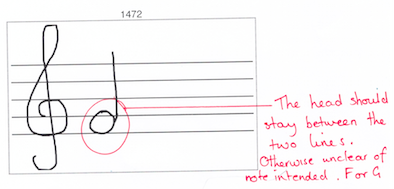
\includegraphics[width=.6\linewidth]{gfx/teacher-notes/mistake-notehead-ambiguous.png}
  \caption{And example of an `ambiguous' minim. It is placed both in a space and on a line}
  \label{fig:mistake-note-ambig}
\end{figure}

\subsubsection{Broken Note Heads}\label{sec:tf-note-head-broken}

\begin{figure}[H]
  \centering
  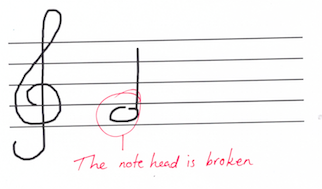
\includegraphics[width=.6\linewidth]{gfx/teacher-notes/mistake-notehead-broken.png}
  \caption{When writing semibreves and minims, it's important to form a full ellipse}
\end{figure}

\subsubsection{Messy Note Heads}\label{sec:tf-note-head-messy}

\begin{figure}[H]
  \centering
  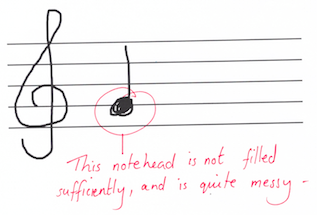
\includegraphics[width=.6\linewidth]{gfx/teacher-notes/mistake-notehead-messy.png}
  \caption{Several children drew solid noteheads rather haphazardly, leaving gaps and giving a messy scribbled effect to the note head}
\end{figure}

\subsubsection{Angled Heads}\label{sec:tf-semibreve-angled}


\begin{figure}[H]
  \centering
  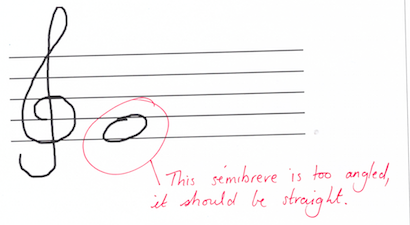
\includegraphics[width=.6\linewidth]{gfx/teacher-notes/mistake-notehead-angled.png}
  \caption{Semibreves are typically wider than minims so any deviation from horizontal appears more pronounced and should be avoided}
\end{figure}

\subsection{Note Stems}

\subsubsection{Stem Angle}\label{sec:tf-stem-angle}

\begin{figure}[H]
  \centering
  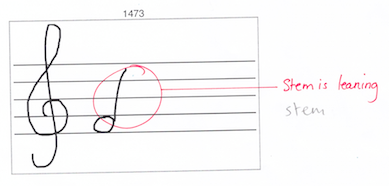
\includegraphics[width=.6\linewidth]{gfx/teacher-notes/mistake-stem-angle.png}
  \caption{}
\end{figure}

\subsubsection{Stem Straightness}\label{sec:tf-stem-straightness}

\begin{figure}[H]
  \centering
  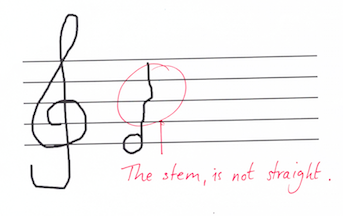
\includegraphics[width=.6\linewidth]{gfx/teacher-notes/mistake-stem-not-straight}
  \caption{}
\end{figure}

\subsubsection{Stem Direction}\label{sec:tf-stem-direction}

\begin{figure}[H]
  \centering
  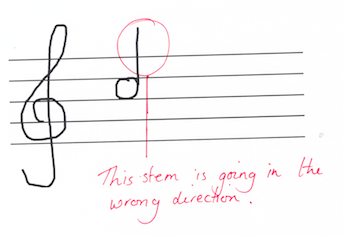
\includegraphics[width=.6\linewidth]{gfx/teacher-notes/mistake-stem-wrong-direction.png}
  \caption{}
\end{figure}

\subsubsection{Stem Side}\label{sec:tf-stem-side}
\todo[inline,color=red]{Manuscript Mistakes - Stem Side}

\subsubsection{Stem Length}\label{sec:tf-stem-length}

\begin{figure}[H]
  \centering
  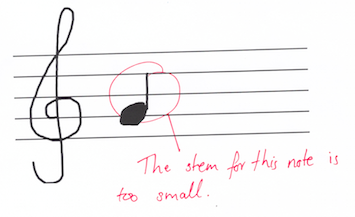
\includegraphics[width=.4\linewidth]{gfx/teacher-notes/mistake-stem-too-short}
  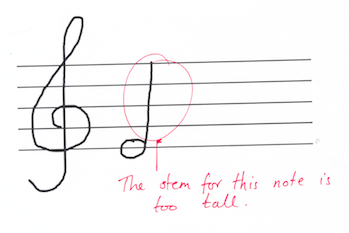
\includegraphics[width=.4\linewidth]{gfx/teacher-notes/mistake-stem-too-long}
  \caption{}
\end{figure}

\subsection{Quaver Tails}

\subsubsection{Quaver Tail Side}\label{sec:tf-quaver-tail-side}

\begin{figure}[H]
  \centering
  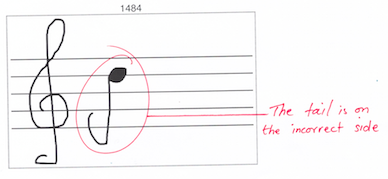
\includegraphics[width=.6\linewidth]{gfx/teacher-notes/mistake-quaver-tail-wrong-side.png}
  \caption{}
\end{figure}

\subsection{Rests}

\subsubsection{Position}\label{sec:tf-rest-position}
Most rests should be centred around the middle staff line. However minim and semibreve rules differ slightly. Minim rests are placed sitting on top of the middle line and semibreve rests are placed sitting below.

\begin{figure}[H]
  \centering
  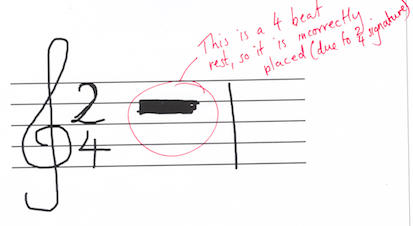
\includegraphics[width=.6\linewidth]{gfx/teacher-notes/mistake-rest-position.png}
  \caption{}
\end{figure}

\subsection{Duration Dots}

\subsubsection{Wrong Side}\label{sec:tf-dot-wrong-side}

\begin{figure}[H]
  \centering
  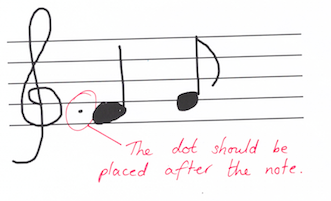
\includegraphics[width=.6\linewidth]{gfx/teacher-notes/mistake-dot-wrong-side.png}
  \caption{}
\end{figure}

\subsection{Accidentals}

\subsubsection{Ambiguous}\label{sec:tf-accidental-ambiguous}

\begin{figure}[H]
  \centering
  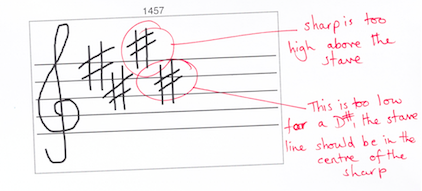
\includegraphics[width=.6\linewidth]{gfx/teacher-notes/mistake-accidental-ambiguous.png}
  \caption{}
\end{figure}

\subsubsection{Wrong Side}\label{sec:tf-accidental-wrong-side}

\begin{figure}[H]
  \centering
  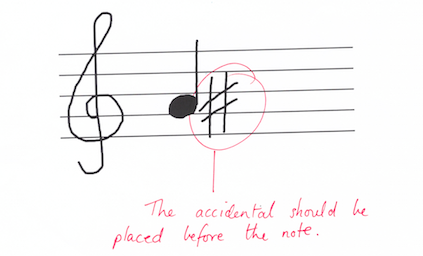
\includegraphics[width=.6\linewidth]{gfx/teacher-notes/mistake-accidental-wrong-side.png}
  \caption{}
\end{figure}

\subsubsection{Wrong Line}\label{sec:tf-accidental-wrong-line}

\begin{figure}[H]
  \centering
  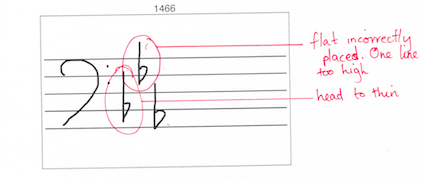
\includegraphics[width=.6\linewidth]{gfx/teacher-notes/mistake-accidental-wrong-line.png}
  \caption{}
\end{figure}

\subsection{Key Signatures}

\subsubsection{Wrong Octave}\label{sec:tf-keysig-octave}

\begin{figure}[H]
  \centering
  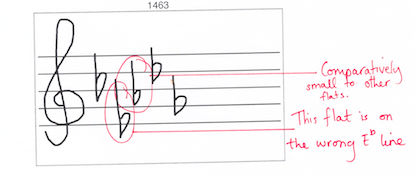
\includegraphics[width=.6\linewidth]{gfx/teacher-notes/mistake-accidental-wrong-octave.png}
  \caption{}
\end{figure}

\subsubsection{Incorrect Order}\label{sec:tf-keysig-order}

\begin{figure}[H]
  \centering
  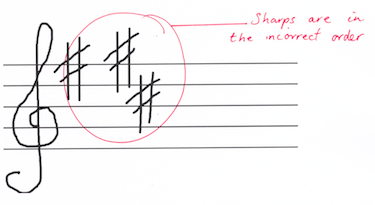
\includegraphics[width=.6\linewidth]{gfx/teacher-notes/mistake-keysig-order.png}
  \caption{}
\end{figure}

\subsubsection{Incorrect Pitch}\label{sec:tf-keysig-incorrect}

\begin{figure}[H]
  \centering
  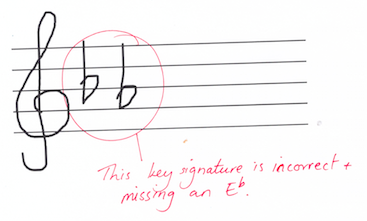
\includegraphics[width=.6\linewidth]{gfx/teacher-notes/mistake-keysignature.png}
  \caption{}
\end{figure}

\subsection{Beats and Timing}

\subsubsection{Too Many Beats}\label{sec:tf-beats-too-many}

\begin{figure}[H]
  \centering
  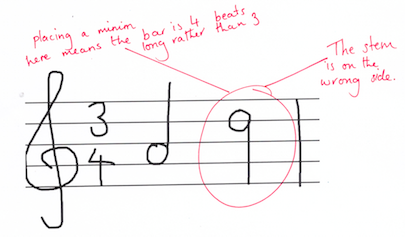
\includegraphics[width=.6\linewidth]{gfx/teacher-notes/mistake-beats-too-many.png}
  \caption{}
\end{figure}

\subsubsection{Too Few Beats}\label{sec:tf-beats-too-few}

\begin{figure}[H]
  \centering
  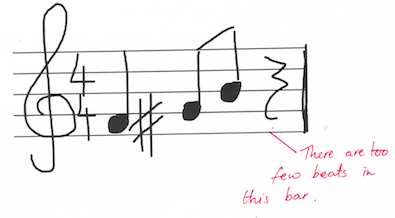
\includegraphics[width=.6\linewidth]{gfx/teacher-notes/mistake-beats-too-few.png}
  \caption{}
\end{figure}




